\chapter{Motivation}
\label{chapter:body}
\thispagestyle{myheadings}

% set this to the location of the figures for this chapter. it may
% also want to be ../Figures/2_Body/ or something. make sure that
% it has a trailing directory separator (i.e., '/')!
\graphicspath{{2_Body/Figures/}}


\section{Concept Development}
Scientists \& Engineers have studied the basic fundamentals governing atoms and electrons; however, a molecule contains too many interactions for modern day computers to fully calculate. As a result, drug development is very slow and expensive. To add on to this, the amount of transistor scaling is reaching a limit as Moore's Law slows down due to circuits approaching fundamental limits. Amdahl's law tells us that adding more processors can only get us so far as even parallelization has its speed limits. Lastly, supercomputers are very power hungry and as a result the more we scale up supercomputers the more exponentially power hungry these systems become. Quantum Computers could significantly extend the ability to simulate the structure and properties of molecules, including how chemicals, drugs, and hormones interact with the human body. Through large scale analytics and machine learning, quantum computing can give more information on gene expression and the origin of mutations which will be beneficial to clinical studies. \newline
\indent There is a variety of quantum computing architectures available such as trapped ions \cite{Blatt:12}, quantum annealing \cite{RevModPhys.80.1061} , superconducting qubits \cite{Paraoanu2014} and in the context of my thesis-single photons \cite{PhysRevLett.104.153602}. Available setups in the market and R\&D involve very large scale setups along with the need of cooling down these systems down to near $0 K$ temperatures which would not be as desirable long term. The utilization of photonic systems would be a worthy competitor in quantum computing technology as they can perform in room temperature with simple optical components and have the potential to be scaled down to on-chip systems. One problem with these systems is that the photons do not interact as easily and this leads to a naturally decoherence-free system but complicates entanglement generation. Photons are not restricted to interactions with nearest neighbours due to their abiility to move freely in free space or in waveguides. In an on-chip system, free photon mobility gives arbitrary interconnections and allows simulations of complex and non-local many-body interactions \cite{aspuru-guzik_photonic_2012}. \newline
\indent This leads us to the mobility of photons allowing us to simulate Quantum Walks through single-photon or multi-photon experiments. Multi-photon experiments provide novel affects in quantum walks. Loop-based architectures have been enabled up to $28$ step discrete walks \cite{PhysRevLett.104.050502}. Our system will essentially have photons going on a Quantum Walk around a 3 node closed system which one can generalize as a quantum walk around a $N$-node circle. Tuning the phase angles in our setup will allow for adjusting the eigenenergies and eigenstates to a close enough threshold that is comparable to the eigenenergies and eigenstates of the chosen simulated molecule which in our case is a Benzene molecule. Also, the concept of having quantum walks around a $N$-node circle allow for photon-photon interaction which is one of the current shortcomings in Optical Quantum Computing that needs to be overcome. Mixing time on the circle increases quadratically faster than a classical random walk \cite{PhysRevA.95.052338}.Success in performing these experiments and simulations will provide a testing ground to scale up our setup to other molecules and provide a framework for potential on-chip integration especially once one is able to keep entangled pairs of photons for a sufficient amount of time.

\newpage

\chapter{System Description}
\section{Experiemental Abstraction}
The following abstraction is what one should experiment when creating a full optical benzene model with our foundation. This abstraction also allows us to form the mathematical model that we will define later on. Note, that the abstraction does not include the inputs for the laser, measurement sites, optical circulators, any other necessary equipment. An optical schematic and laboratory picture of a single optical triport setup will be presented in the section following this one. \newline
\begin{figure}[H]
    \centering
    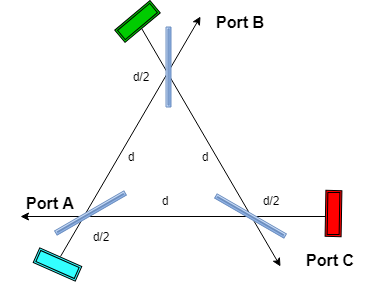
\includegraphics{three_port_diagram.png}
    \caption{The Directionally-Unbiased Optical Three port. The thin blue rectangles represent the directionally-unbiased beam splitters. The colored rectangles represent the mirror units which contain a phase shifter and a mirror.}
    \label{fig:my_label}
\end{figure}
\indent The optical multiport is in the arrangement of a triangular 3-port (as shown above) which consists of phase shifters, mirrors, and beam splitters at each of the three ports. The beam splitters in the multiport are directionally unbiased which means light going into a port can also have the option to exit out the same port. Since Benzene has 6 vertices of carbon, there will be 6 triports connected to one another. Two ports of the triport will connect to two ports of another triport to represent a double-bond connection and the remaining single port connections will represent a single-bond. 
The unbiased multiport is distinguished from regular beam splitters and multiports by their high levels of summetry and reversibility of the photon's movement through the system which make them more distinct from ther standard devices. Here in the abstraction, the ports are an equivalent distance $d$ apart. The labeled ports will allow us to describe a mathematical standard basis of vectors when constructing the Hamiltonian of the system. In the case of this thesis, I will choose $B$ and $C$ to be the two-ports to make the \textit{double-bond} connection to the $B$ and $C$ port of an adjacent triport and port $A$ to be used for representing the \textit{single-bond} connection to the $A$ port of the adjacent triport. Therefore, there will be three edges with double bonds and three edges with single bonds which will correspond to a single bond. The abstract construction of the optical benzene will be modeled mathematically for the construction of the Hamiltonian and its associated eigenvalues and eigenstates of the system. 
\begin{figure}[H]
    \centering
    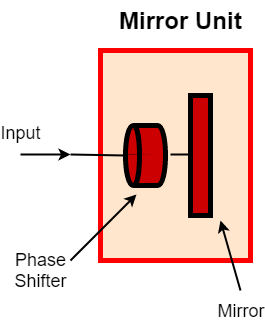
\includegraphics[scale=0.6]{mirror_unit_01.png}
    \caption{The Mirror Unit which consists of a phase shifter and a mirror. The distance between each beam splitter and the adjacent mirror is half the distance $d$ between one beam splitter and the other. The phase shifter will be helpful in controlling the phase of the photons and interference of photon paths.}
    \label{fig:my_label}
\end{figure}

\begin{figure}[H]
    \centering
    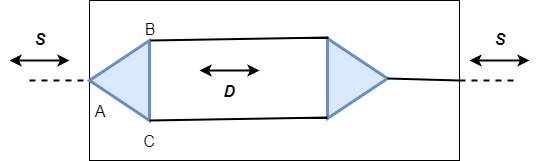
\includegraphics[scale=0.6]{unit_multiport_cell_diagram_2.png}
    \caption{The Unit Cell of two directionally-unbiased triports connected to represent a double bond of a benzene system and the other end representing a single bond. Three of these unit cells will make up the optical benzene setup. $S$ (single-bond state) and $D$ (double-bond state) will later on be used to represent in bond states of the cell in our Hamiltonian model.}
    \label{fig:my_label}
\end{figure}

\begin{figure}[H]
\centering
\begin{subfigure}{.5\textwidth}
  \centering
  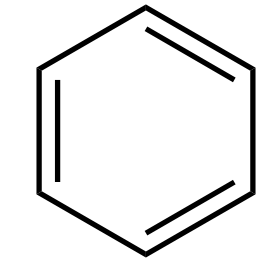
\includegraphics[width=.4\linewidth]{benzene_molecule.png}
  \caption{Actual Benzene Molecule}
  \label{fig:sub1}
\end{subfigure}%
\begin{subfigure}{.5\textwidth}
  \centering
  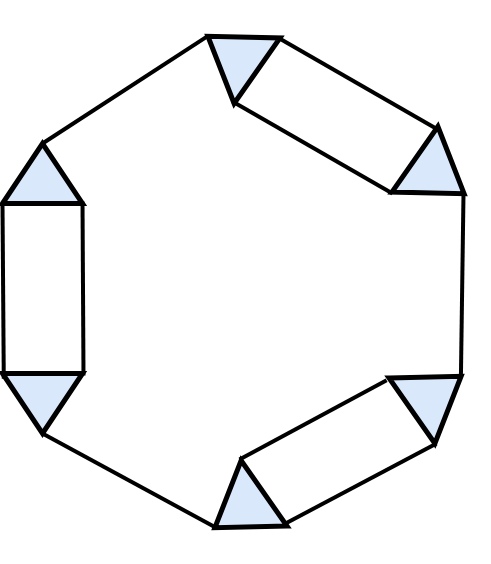
\includegraphics[width=.4\linewidth]{optical_benzene_diagram_01.png}
  \caption{Optical Benzene System}
  \label{fig:sub2}
\end{subfigure}
\caption{Side by Side of a Benzene molecule ($C_{6}H_{6}$) with the abstraction of our Optical Benzene molecule. Photons injected into the optical system will undergo quantum random walks around the system analagous to the electron movement in the aromatic ring of a Benzene molecule}
\label{fig:test}
\end{figure}

\newpage
\section{Laboratory Setup of Single Optical Triport}

\begin{figure}[H]
    \centering
    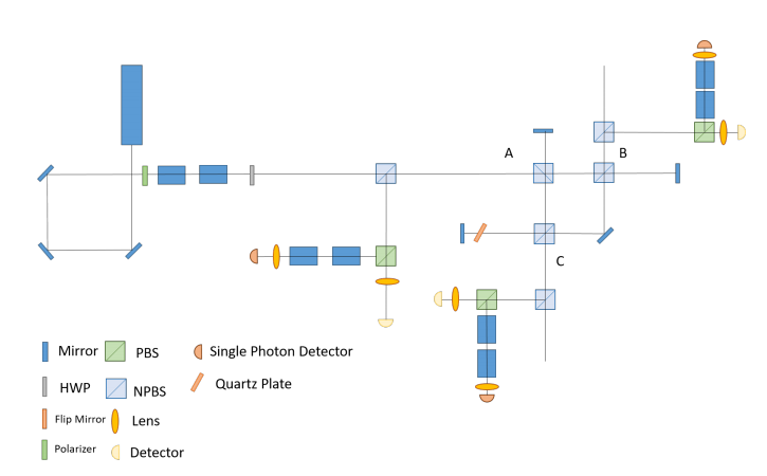
\includegraphics[scale=0.8]{2_Body/Figures/updated_setup.png}
    \caption{Optical Schematic of a Single Optical Triport}
    \label{fig:my_label}
\end{figure}
Our 633 nm laser delivers a stream of photons that bound around mirrors and into polarizing beam splitters which allow us to prepare the input states of the photons before they enter the field of three beam splitters which represent the three ports of the triport as shown in Fig. 4.1. The mirror units in this schematic only contain a mirror as the mirrors are laying on a translational stage which will act as the phase shifter in our setup. The beam will eventually lead out into a detector positioned a bit off in the setup. This setup seems more complicated than our abstracted setup due to practice problems arising such as attempting to allign a beam splitters at angles other than $45$ or $90$ degrees.

\section{Software Implementation}
Software implementation for the simulation and numerical analysis of the optical Benzene model is done on Python 3.6 with assistance with the QuTip Python Quantum Computing Toolbox. \newline
\textbf{Optical Benzene Numerical Analysis Class}
\begin{enumerate}
    \item Uses port phase angle $\phi$ as tunable parameter
    \item Sets the amplitudes of the unitary matrix for a three-port device
    \item Includes Pandas Options for readable matrix outputs
    \item Constructs Hamiltonian from Unitary Matrix
    \item Solves for Eigenvalues and Eigenvectors
    \item Constructs Photon movement Projected out Hamiltonian and associated eigenvaleus and eigenvectors
\end{enumerate}
\textbf{Script for plotting Eigenspectrum and Eigenstates for Optical Benzene} 
\begin{enumerate}
    \item Creates plots of the Eigenvalues (Eigenenergies) as a function of the phase angle $\phi$ for all Eigenvalues for either Hamiltonian
    \item Creates plots of the probability amplitudes of the Eigenstates as a function of the state for a given eigenvalue at a given phase angle $\phi$
\end{enumerate}

 
 
 
 
 
 
 
 
 
 
 
 
 \chapter{Optical Benzene Model}
 \section{Basis Formulation}
 The Hamiltonian provides the energy dynamics and information of a quantum mechanical system. By solving the Time-Independent Schrodinger Equation:
 \begin{equation}
     H\ket{\psi_{n}} = E_{n} \ket{\psi_{n}}
 \end{equation}
 one may arrive at the eigenvalues $E_{n} $ which correspond to the energy levels of a molecular system and the eigenenergies have associated eigenvectors $\ket{\psi_{n}}$ which describe the associated state of the system i.e. position, momentum etc.  \newline
 I define a basis for the multiport connected benzene system. The unit cells of the connected triports will be defined by the following $12 \times 12$ Hilbert space:
 \begin{equation}
     \mathcal{H} = \ket{n} \otimes \ket{M} \otimes \ket{B}
 \end{equation}
 Where $n \in \{1,2,3\}$ represent the unit cell index corresponding to the 3 unit cells (6 triports) of the optical benzene, $m \in \{L, R\}$ represents the left and right moving states of a photon in the system, and $B \in \{S, D\}$ represent the single and double states of a photons position within a unit cell. Note that this system is cyclic with $n \mod 3$.
 \section{States of the System}
 \subsection{Triport Representation}
 The Ports $A, B, C$ of the $3$-port optical multiport form a $3$-dimensional standard basis:
 \begin{equation}
    \ket{A} = \begin{pmatrix}
    1 \\
    0 \\
    0 \end{pmatrix}
    ,
    \ket{B} = \begin{pmatrix}
    0 \\
    1 \\
    0 \end{pmatrix}
    ,
    \ket{C} = \begin{pmatrix}
    0 \\
    0 \\
    1 \end{pmatrix}
\end{equation}

\subsection{Unit Cell Representation}
Based on Fig 3.3 and the the Hilbert Space of this system, the single bond state $S$ is taken to be port $A$ of a optical triport and the double bond state $D$ is taken to be port $B$ and $C$ of a optical triport. Using Eq. 4.3 one may define the double bond states of the $B$ space as the following:
\begin{equation}
    \ket{S} = \ket{A} = \begin{pmatrix}
    1 \\ 0 \\ 0 \end{pmatrix}
\end{equation}
\begin{equation}
    \ket{D} = \frac{1}{\sqrt{2}}(\ket{B}+\ket{C}) = \frac{1}{\sqrt{2}}
    \begin{pmatrix}
    0 \\ 1 \\ 1 \end{pmatrix}
\end{equation}

One may also reduce the representation of the bond states to a $2$-dimensional standard basis which will be used for a specific case later on:
\begin{equation}
    \ket{S} = \begin{pmatrix} 1 \\ 0 \end{pmatrix},
    \ket{D} = \begin{pmatrix} 0 \\ 1 \end{pmatrix}
\end{equation}


\section{Directionally-Unbiased Optical Three-Ports}
It is important to derive the photon dynamics within a single directionally unbiased optical three-port device In order to this, the unitary matrix that describe the transitions from one port to another port in a three-port must be derived. \cite{PhysRevA.93.043845}. 
\newline
Assume that a photon into Port A. Due to the reflection symmetry in the input direction, the exit amplitudes for the other two ports should be equal. So given an input state $\ket{\psi_{in}} = \ket{A}$ then the output is of the form:
\begin{equation}
    \ket{\psi_{out}} = a\ket{A} + b(\ket{B} + \ket{C})
\end{equation}
With complex amplitudes $a$ and $b$. Repeating the argument for inputs $B$ and $C$ , the transition matrix $V$ is of the form :
\begin{equation}
    V = \begin{pmatrix}
    a & b & b \\
    b & a & b \\
    b & b & a 
    \end{pmatrix}
\end{equation}
The matrix is unitary, therefore $V \cdot V^{\dagger} = I$ , the diagonal and off-diagonal entries must satisfy the normalization constraints: 
\begin{equation}
    |a|^2 + 2|b|^2 = 1 , 2Re(ab^{*}) + |b|^2 = 0 
\end{equation}
Define the following:
\begin{equation}
    a = \alpha e^{i\phi_{a}}, b = \beta e^{i\phi_{b}}
\end{equation}
\begin{equation}
    \phi = \phi_{b} - \phi_{a}
\end{equation}
Solving for Eqn (8) and (9) gives:
\begin{equation}
    \alpha = \sqrt{\frac{1}{1 + 8\cos^{2}\phi}}
\end{equation}
\begin{equation}
    \beta = -2 \sqrt{\frac{\cos^{2}\phi}{1+8\cos^{2}\phi}}
\end{equation}
Putting it all together $V$ becomes of the following form:
\begin{equation}
    V = \frac{e^{i\phi_{a}}}{\sqrt{1+8\cos^{2} \phi}} 
    \begin{pmatrix}
    1 & -2 e^{-i\phi}\cos\phi & -2e^{-i\phi}\cos\phi \\
    -2e^{-i\phi}\cos\phi & 1 & -2e^{-i\phi}\cos\phi \\
    -2e^{-i\phi}\cos\phi & -2e^{-i\phi}\cos\phi & 1 
    \end{pmatrix}
\end{equation}
The special case of $\phi = 0$ gives
\begin{equation}
    V(\phi_{a}) = \frac{1}{3}e^{i\phi_{a}} 
    \begin{pmatrix}
    1 & -2 & -2 \\
    -2 & 1 & -2 \\
    -2 & -2 & 1 \end{pmatrix}
\end{equation} 
More generally, for the context of this research, all 3 ports are set equal to one another and set as a single tunable paramter $\phi$, provides a unitary matrix $U$ of the following form: 
\begin{equation}
    \phi = \phi_{A} = \phi_{B} = \phi_{C}
\end{equation}
\begin{equation}
    U = \frac{e^{i\phi}}{2+ie^{i\phi}}
    \begin{pmatrix}
    1 & ie^{-i\phi} - 1 & ie^{-i\phi} - 1 \\
    ie^{-i\phi} - 1 & 1 & ie^{-i\phi} - 1 \\
    ie^{-i\phi} - 1 & ie^{-i\phi} - 1 & 1 \end{pmatrix}
\end{equation}
 
 
\section{The Full General Model}
\subsection{System Interactions}
Given our full $12 \times 12$ Hilbert Space and the Unitary matrix for a single three-port, we now derive the transitions for a photon within the optical three-port connected benzene model. \newline

The transitions within the optical benzene system described by the three state spaces-- unit cell index (cyclic $\mod 3$, $n-1, n, n+1$), right/left moving ($R/L$) and bond sites ($S/D$) are given as the following: 

\begin{enumerate}
    \item $SR \rightarrow DR,  n \rightarrow n + 1, n+1 \rightarrow n-1 , n-1 \rightarrow n$
    \item $DR \rightarrow SR, n, n+1, n-1$ fixed
    \item $SR \rightarrow SL, n , n+1, n-1$ fixed
    \item $DR \rightarrow DL , n , n+1, n-1$ fixed
    \item $SL \rightarrow DL, n, n+1, n-1$ fixed
    \item $DL \rightarrow SL, n \rightarrow n-1, n+1 \rightarrow n, n-1\rightarrow n+1$
    \item $SL \rightarrow SR, n, n+1, n-1$ fixed
    \item $DL \rightarrow DR, n, n+1, n-1$ fixed
\end{enumerate}

\subsection{Transition Amplitudes}



First, for simplicity we define new variables for the amplitude value and unitary matrix scaling term in Eq. (4.17):
\begin{equation}
    \beta =  \frac{e^{i\phi}}{2+ie^{i\phi}}
\end{equation}
\begin{equation}
    \rho = ie^{-i\phi} - 1
\end{equation}

Transition Amplitudes between the bond sites in terms of the bond states are as follows ($\beta$ appears in all as it is a factor outside the unitary matrix): 
\begin{equation}
    S \Longleftrightarrow S \rightarrow \braket{A|A} = \beta
\end{equation}
\begin{equation}
    S \Longleftrightarrow D \rightarrow \frac{1}{\sqrt{2}} \braket{A|B+C} = \frac{2}{\sqrt{2}}\rho \beta = \sqrt{2} \rho \beta
\end{equation}
\begin{equation}
    D \Longleftrightarrow D \rightarrow \frac{1}{2} \braket{B+C|B+C} = \frac{1}{2} (\braket{B|B} + \braket{C|C} + 2\operatorname{Re}\braket{B|C}) = \beta (1 + \rho)
\end{equation}
\newpage
\subsection{Full Unitary Matrix Formulation}
Given these amplitudes and transition information, we can now construct the full 12 by 12 Unitary matrix for a state $\ket{B,M,n}$ where $B \in \{S, D\}$ (bond states) , $M \in \{L, R\}$ (motion of photon - left or right), $n \in \{1,2,3\}$ (unit cell index). Due to cyclical behaviour one can create a 3 by 3 block circulant matrix where the block matrices are 4 by 4:
\begin{equation}
    \hat{U} = \beta \begin{pmatrix}
    \Lambda_{1} & \Lambda_{2} & \Lambda_{3} \\
    \Lambda_{3} & \Lambda_{1} & \Lambda_{2} \\
    \Lambda_{2} & \Lambda_{3} & \Lambda_{1} \end{pmatrix}
    \end{equation}
Where $\Lambda_{1}, \Lambda_{2}, \Lambda_{3}$ represent the following matrix blocks:
\begin{equation}
    \Lambda_{1} = 
    \begin{blockarray}{ccccc}
    \ket{SLn} & \ket{SRn} & \ket{DLn} & \ket{DRn}\\
    \begin{block}{(cccc)c}
     0 & 1 & 0 & 0 & \ket{SLn}\\
    1 & 0 & 0 & \sqrt{2}\rho & \ket{SRn}\\
    \sqrt{2}\rho & 0 & 0 & 1+\rho & \ket{DLn} \\
    0 & 0 & 1+\rho & 0 & \ket{DRn} \\
    \end{block}
    \end{blockarray}
\end{equation}

\begin{equation}
    \Lambda_{2} = 
    \begin{blockarray}{ccccc}
    \ket{SLn} & \ket{SRn} & \ket{DLn} & \ket{DRn}\\
    \begin{block}{(cccc)c}
    0 & 0 & \sqrt{2}\rho & 0 & \ket{SLn-1} \\
    0 & 0 & 0 & 0 & \ket{SRn-1} \\
    0 & 0 & 0 & 0 & \ket{DLn-1} \\
    0 & 0 & 0 & 0 & \ket{DRn-1} \\
    \end{block}
    \end{blockarray}
\end{equation}

\begin{equation}
    \Lambda_{3} = 
    \begin{blockarray}{ccccc}
    \ket{SLn} & \ket{SRn} & \ket{DLn} & \ket{DRn}\\
    \begin{block}{(cccc)c}
    0 & 0 & 0 & 0 & \ket{SLn+1} \\
    0 & 0 & 0 & 0 & \ket{SRn+1} \\
    0 & 0 & 0 & 0 & \ket{DLn+1} \\
    0 & \sqrt{2}\rho & 0 & 0 & \ket{DRn+1} \\
    \end{block}
    \end{blockarray}
\end{equation}
\newpage
\subsection{Full Hamiltonian Model}
In order to obtain the Hamiltonian from the Unitary Matrix, we solve the Time-Dependent Schrodinger Equation:
\begin{equation}
    \frac{d\ket{\psi}_{BMn}}{dt} = -i\frac{\hat{H(t)}}{\hbar}
\end{equation}
The Unitary Operator $\hat{U}$ is a wave equation solution and describes the time-evolution of the eigenstates expressed as:
\begin{equation}
    \hat{U} = e^{-iHT/\hbar}
\end{equation}
Where $T$ is time and $\hbar$ is the reduced Planck's constant. For simplicity we will set $T = \hbar = 1$ leading to:
\begin{equation}
    U = e^{-iH}
\end{equation}
Given that $U$ and $H$ are both matrices, we take the matrix logarithm operation on both sides (can be computed through various numerical approximations and method, see Appendix A.2 for more information) and this provides the Hamiltonian as the following:
\begin{equation}
    H = i\ln U
\end{equation}
One can verify analytically that our Unitary matrix $U$ holds the Unitary Condition:
\begin{equation}
    UU^{\dagger} = I
\end{equation}
Afterwards, one can verify numerically that the Hamiltonian holds the Hermiticity Condition:
\begin{equation}
    H = H^{\dagger}
\end{equation}
\newpage
\section{Reduced General Model without Direction of Movement}
Given the 6 Carbon atom nature of a Benzene molecule, there is going to be a set of 6 energy levels and energy states and thus we'd like to also have a Hamiltonian model that is reduced down to that size. We do this by projecting out the $M$ vector space that describes the movement of a photon in the system as either leftmoving $L$ or rightmoving $R$.
\subsection{Projection Operator}
In order to reduce our Hilbert Space, we define a projection operator that when acted upon the full 12 by 12 vector space, gets reduced down to a 6 by 6 space via the Hamiltonian being projected onto the diagonal subspace of the left-and right-moving modes. 
\begin{equation}
     \mathcal{H} = \ket{n} \otimes \ket{M} \otimes \ket{D} \rightarrow \mathcal{H'} = \ket{n} \otimes \ket{B}
\end{equation}
\begin{equation}
    \hat{P} = \sum_{Bond\&Position Subspace} \ket{m} \bra{m}
\end{equation}
Given a state of the form $\ket{B,M,n}$ then the Projection operator is a superposition of left and right moving states that multiply across the Hamiltonian to form the matrix elements of the reduced Hamiltonian: 
\begin{equation}
    P = \frac{1}{\sqrt{2}} (\ket{B,L,n}\bra{B,n,L} + \ket{B,R,n}\bra{B,R,n})
\end{equation}
\subsection{Reduced Hamiltonian Model}
Using the Projection Operator above, one can apply it to our full Hamiltonian matrix by multiplying $H$ on the left and right side with the hermitian conjugate of the projection operator and the projection operator respectively to obtain the reduced Hamiltonain $H'$:
\begin{equation}
    H' = P^{\dagger}HP
\end{equation}

\chapter{Eigendecomposition of the System}
\section{Eigenvalues of Full Hamiltonian}
In order to obtain the eigenenergies (eigenvalues) of the Hamiltonian, we solve the eigenvalue/eigenvector problem that arises from the Time-Independent Schrodinger Equation:
\begin{equation}
    \hat{H}(\phi)\ket{B,M,n} = E_{i}(\phi)\ket{B,M,n}
\end{equation}
Where $i = 1,2,\hdots ,12$ and $\phi$ is the phase angle parameter for the multiports. \newline
The eigenvalues arise from the following expression where one must solve for $E_{i}$:
\begin{equation}
    \det (H - E_{i}I) = 0
\end{equation}
\section{Eigenstates of Full Hamiltonian}
Using the derived eigenvalues, one may solve the associated eigenstates (eigenvectors) of the Hamiltonian by plugging in the individual eigenvalues into Eq. (5.1) and solving for the values of the eigenvector by inspection or via Gaussian Elimination:
\begin{equation}
    (H - E_{i}I)\ket{\psi}_{BMn}^{(i)} = 0 
\end{equation}
Eigenstates must be normalized after being obtained:
\begin{equation}
    |\ket{\psi}|^2 = 1
\end{equation}
\section{Eigenanalysis for $\phi = \pi/2$}
In a series of a few test cases of $\phi$ phase angles, we start with eigenanalysis for $\pi/2$ which produces some interesting results of the system collapsing to two 6-fold degenerate energy levels (full Eigenspectrum plot shown later in this thesis)
\subsection{Parameter Values}
Plugging in our phase angle of $\pi/2$ into our parameter values $\beta, \rho$ that denote the transition amplitudes:
\begin{equation}
    \beta(\pi/2) = \frac{e^{i\pi/2}}{2+ie^{i\pi/2}} = i 
\end{equation}
\begin{equation}
    \rho(\pi/2) = ie^{-i\pi/2} - 1 = 0
\end{equation}
\subsection{Matrix Block Values}
Given that the submatrices $\Lambda_{2}, \Lambda_{3}$ only contain one value which is $\sqrt{2}\rho$ and $\rho(\pi/2)$ is $0$ , these submatrices become $0$-matrix blocks leaving the $\Lambda_{1}$ submatrix as follows:
\begin{equation}
    \Lambda_{1}(\pi/2) = \begin{pmatrix} 0 & 1 & 0 & 0 \\ 1 & 0 & 0 & 0 \\ 0 & 0 & 0 & 1 \\ 0 & 0 & 1 & 0 \end{pmatrix},  \Lambda_{2} = \Lambda_{3} = 0 
\end{equation}
Given that other blocks are 0, one can exploit the symmetry of the matrix and find the eigenvalues of the $\Lambda_{1}$ block and extend it two more times. \newline 
It is evident that $\Lambda_{1}$ can be diagonalized and thus there exists a matrix $S$ such that:
\begin{equation}
    D = S\Lambda_{1}S^{-1}
\end{equation}
Where $D$ is diagonalized matrix of $\Lambda_{1}$, this is found to be:
\begin{equation}
    D = \begin{pmatrix} -1& 0 & 0 & 0 \\ 0 & -1 & 0 & 0 \\ 0 & 0 & 1 & 0 \\ 0 & 0 & 0 & 1 \end{pmatrix}
\end{equation}
\subsection{Eigenvalues}
If a matrix is diagonal, then the elements $D_{ii}$ along the main diagonal are the eigenvalues of the matrix:
\begin{equation}
    E_{1,2,3,4,5,6}^{U(\pi/2)} = -i = e^{-i\pi/2}
\end{equation}
\begin{equation}
    E_{7,8,9,10,11,12}^{U(\pi/2)} = i = e^{i\pi/2}
\end{equation}
Now we take the natural log of each of the eigenvalues to produce the eigenvalues of the Hamiltonian:
\begin{equation}
    E_{1,2,3,4,5,6}^{H(\pi/2)} = -\pi/2
\end{equation}
\begin{equation}
    E_{7,8,9,10,11,12}^{H(\pi/2)} = \pi/2
\end{equation}
\subsection{Eigenstates}
The pair of 6-fold degeneracies at $\pm \pi/2$ produce eigenstates that show the photon is in a superposition of left or right moving within a bond site and unit cell position along the entire system which gives rises to non-stationary states. \newline
This is evident from the Unitary Transformation showing only transitions between Left and Right Modes within a fixed unitcell and bond site.
\begin{table}[h]
    \centering
    \begin{tabular}{c|c}
        \hline 
        Eigenvalue $E$ & Eigenstate $\ket{B,M,n}$ \\
        \hline
        \multirow{3}{*}{$-\pi/2$} & $\frac{1}{\sqrt{2}}$ \Big[$(1,1,0,0,\hdots,0)^{T}, (0,0,1,1,\hdots,0)^{T},$ \\
        & $(0,0,0,0,1,1,\hdots, 0)^{T}, (0,0,0,0,0,0,1,1,\hdots, 0)^{T}$ \\
        & $(0,0,0,0,0,0,0,0,1,1,\hdots,0)^{T}, (0,\hdots,1,1)^{T}$ \Big]\\ \hline
        \multirow{3}{*}{$\pi/2$} & $\frac{1}{\sqrt{2}}$ \Big[$(0,0,1,-1,\hdots, 0)^{T}, (0,0,0,0,0,0,1,-1,\hdots,0)^{T}$ \\ & $(1,-1,\hdots, 0)^{T}, (0, \hdots,1, -1, 0, 0)^{T}$\\
        \\ & $(0,0,0,0, 1,-1,\hdots, 0)^{T}, (0, \hdots, 1, -1)^{T} $ \Big] \\
        \hline
    \end{tabular}
    \caption{Corresponding Eigenstates to the Eigenvalues for $H(\pi/2)$ }
    \label{tab:my_label}
\end{table} \newpage
\subsection{Qualitative Description}
For $E = -\pi/2$, each eigenstate is a steady state with the average photon reflecting from left to right within a fixed unit cell and fixed bond site. \newline
For $E = \pi/2$, each eigenstate is a steady state with the average photon reflecting right to left within a fixed unit cell and fixed bond site. 
\section{Eigenanalysis for $\phi = 3\pi/2$}
Now we traverse to the other side of the phase plane and look at $\phi = 3\pi/2$ which produces a more "opposite" effect than that of $\phi = \pi/2$. The system produces a set of six 2-fold degenerate energy levels. 
\subsection{Parameter Values}
Pluggin in $\phi = 3\pi/2$ we get:
\begin{equation}
    \beta(3\pi/2) = -\frac{i}{3}
\end{equation}
\begin{equation}
    \rho(3\pi/2) = -2 
\end{equation}
\subsection{Matrix Block Values}
Plugging in the values above into the matrix blocks of the Unitary Matrix, we get the following:
\begin{equation}
     \Lambda_{1}(3\pi/2)  = \begin{pmatrix} 0 & 1 & 0 & 0 \\ 1 & 0 & 0 & -2\sqrt{2} \\ -2\sqrt{2} & 0 & 0 & -1 \\ 0 & 0 & -1 & 0 \end{pmatrix}
\end{equation}
\begin{equation}
    \Lambda_{2}(3\pi/2) = \begin{pmatrix} 0 & 0 & -2\sqrt{2} & 0 \\ 0 & 0 & 0 & 0 \\ 0 & 0 & 0 & 0 \\ 0 & 0 & 0 & 0 \end{pmatrix} 
    , \Lambda_{3} (3\pi/2) = \begin{pmatrix} 0 & 0 & 0 & 0 \\ 0 & 0 & 0 & 0 \\ 0 & 0 & 0 & 0 \\ 0 & -2\sqrt{2} & 0 & 0 \end{pmatrix}
\end{equation}
Due to the size and complexity of the matrix we define the Unitary Matrix as a sum of Kronecker Products in terms of some matrix $P$:
\begin{equation}
    P = \begin{pmatrix} 0 & 1 & 0 \\ 0 & 0 & 1 \\ 1 & 0 & 0 \end{pmatrix}
\end{equation}
\begin{equation}
    3iU = I \otimes \Lambda_{1} + P \otimes \Lambda_{2} + P^{2} \otimes \Lambda_{3}
\end{equation}
\subsection{Eigenvalues}
It is evident that $\Lambda_{2}$ and $\Lambda_{3}$ commute and are both nilpotent matrices ($N^{k} = 0$ for some square matrix $N$ and integer $k$). his infers that $P \otimes \Lambda_{2}$ and $P^2 \otimes \Lambda_{3}$ are commuting nilpotent matrices. This follows that $P \otimes \Lambda_{2} + P^{2} \otimes \Lambda_{3}$ is a nilpotent matrix and by inspection the eigengvalue is $0$ . It satisfies $(P \otimes \Lambda_{2} + P^{2} \otimes \Lambda_{3})^2 = 0 $.
We require an invertible matrix $S$ (columns are eigenvectors) to diagonalize $\Lambda_{1}$ such that we produce a diagonal matrix $D$:
\begin{equation}
    D = S^{-1}\Lambda_{1}S
\end{equation}
The eigenvalues of $\Lambda_{1}$ are 4 distinct and complex valued roots of the characteristic polynomial: 
\begin{equation}
    p(x) = x^4 - 2x^2 + 9
\end{equation}
Let $V = 3iU$ for simplicity
\begin{eqnarray}
    (I \otimes S)^{-1}V (I \otimes S) = 
    \begin{pmatrix}
    S\Lambda_{1}S^{-1} & S\Lambda_{2}S^{-1} & S\Lambda_{3}S^{-1} \\
    S\Lambda_{3}S^{-1} & S\Lambda_{1}S^{-1} & S\Lambda_{2} S^{-1} \\
    S\Lambda_{2}S^{-1} & S\Lambda_{3}S^{-1} & S\Lambda_{1}S^{-1} 
    \end{pmatrix} \\
    = \begin{pmatrix}
    D & M_{2} & M_{3} \\
    M_{3} & D & M_{2} \\
    M_{2} & M_{3} & D
    \end{pmatrix} \\
    = I \otimes D + P \otimes M_{2} + P^{2} \otimes M_{3}
\end{eqnarray}
Solve the characteristic polynomial $p(x) = x^4 - 2x^2 + 9$ \newline
Let $w = x^2, w^2 = x^4$ and solve the substituted polynomial:
\begin{equation}
    w^2 - 2w+ 9 =0
\end{equation}
\begin{equation}
    w = 1 \pm 2\sqrt{2}i
\end{equation}
\begin{equation}
    x^2 = 1 \pm 2\sqrt{2}i
\end{equation}
Let $x = u + iv$
\begin{eqnarray}
    (u + iv)^2 = 1 \pm 2\sqrt{2}i \\
     u^2 - v^2 + 2iuv = 1 \pm 2\sqrt{2}i 
\end{eqnarray}
\begin{equation}
    \begin{pmatrix} u ^2  - v^2  =1 \\ 2uv = \pm \sqrt{2} \end{pmatrix} \rightarrow v = \pm 1 , u = \pm \sqrt{2}
\end{equation}
Therefore the roots of the characteristic polynomiam $p(x)$ for $\Lambda_{1}$ are:
\begin{equation}
    x = \sqrt{2} + i, -\sqrt{2} - i, -\sqrt{2} + i, \sqrt{2} - i
\end{equation}
With the following eigenvector space:
\begin{equation}
    \Vec{v} = \left\{   \begin{pmatrix} i \\ -1+ \sqrt{2}i \\ -i - \sqrt{2} \\ 1 \end{pmatrix} , 
    \begin{pmatrix}
    i \\ 1  - \sqrt{2}i \\ i + \sqrt{2} \\ 1 \end{pmatrix}
    \begin{pmatrix}
    -i \\ 1 + \sqrt{2}i \\ -i + \sqrt{2} \\ 1 \end{pmatrix}
    \begin{pmatrix}
    - i \\ -1 - \sqrt{2}i \\ i - \sqrt{2} \\ 1 \end{pmatrix}
    \right\}
\end{equation}
The eigenspace above makes up the matrix $S$ and the diagonal matrix $D$ is given by the 4 roots of the characteristic polynomial.
\begin{equation}
    S = \begin{pmatrix}
    -i & -i& i & i \\
    1+\sqrt{2}i & -1 - \sqrt{2}i & 1 - \sqrt{2}i & -1 + \sqrt{2}i \\
    \sqrt{2} - i & - \sqrt{2} + i & \sqrt{2} + i & -\sqrt{2} - i \\
    1 & 1 & 1 & 1 \end{pmatrix}
\end{equation}
\begin{equation}
    D = \begin{pmatrix}
    - \sqrt{2} + i & 0 & 0 & 0 \\
    0 & \sqrt{2} - i & 0 & 0 \\
    0 & 0 & - \sqrt{2} - i & 0 \\
    0 & 0 & 0 & \sqrt{2} + i \end{pmatrix}
\end{equation}
Since $\Lambda_{2}$ and $\Lambda_{3}$ are non-diagonizable , we find a Jordan Normal form them
There exists a matrix $M_{2}$ and $M_{3}$ such that $\Lambda_{2} = SM_{2}S^{-1}$ and $\Lambda_{3} = SM_{3}S^{-1}$
\begin{equation}
    \det (\Lambda_{2} - xI) = \det \left( \begin{pmatrix}
    0 & -x & -2\sqrt{2} & 0 \\
    -x & 0 & 0 & 0 \\
    0 & 0 & -x & 0 \\
    0 & 0 & 0 & -x \end{pmatrix} \right) = \det \begin{pmatrix} A & B \\ C & D \end{pmatrix}
\end{equation}
Since $C$ and $D$ commute:
\begin{equation}
    \det (\Lambda_{2} - xI) = -\det ( AD - BC) = -\det \begin{pmatrix} 0 & x^2 \\ x^2 & 0 \end{pmatrix}  = x^{4} = 0 
\end{equation}
Therefore there is one eigenvalue with a value of $0$ with multiplicity $4$ \newline
Via gaussian elimination one can find the matrix $S$ and corresponding $S^{-1}$ to be
\begin{equation}
    S = \begin{pmatrix} 0 & 0 & 1 & 0 \\ 0 & 1 & 0 & 0 \\ 0 & 0 & 0 & -\frac{1}{2\sqrt{2}} \\ 1 & 0 & 0 & 0 \end{pmatrix}
\end{equation}
\begin{equation}
    S^{-1} = \begin{pmatrix} 0 & 0 & 0 & 1 \\ 0 & 1 & 0 & 0 \\ 1 &0&0 &0 \\ 0 & 0 & -2\sqrt{2} & 0 \end{pmatrix}
\end{equation}
\begin{equation}
    M_{2} = S\Lambda_{2}S^{-1} = \begin{pmatrix} 0 & 0 & 0 & 0 \\ 0 & 0 & 0 & 0 \\ 0 & 0 & 1 & 0 \\ 0 & 0&0&0 \end{pmatrix}
\end{equation}
Similarly one can do the same for $\Lambda_{3}$:
\begin{equation}
    S = \begin{pmatrix} 0 & 0 & 0 & 1 \\ 0 & -\frac{1}{2\sqrt{2}} & 0 & 0 \\ 0 & 0 & 1 & 0 \\ 1 & 0 & 0 & 0 \end{pmatrix}, S^{-1} = \begin{pmatrix} 0 & 0 & 0 & 1 \\ 0 & -2\sqrt{2} & 0 & 0 \\ 0 & 0 & 1 & 0 \\ 1 & 0 & 0 & 0 \end{pmatrix}
\end{equation}
\begin{equation}
    M_{3} = S\Lambda_{3}S^{-1} = \begin{pmatrix} 0 & 1 & 0 & 0 \\ 0 & 0 & 0 & 0 \\ 0 & 0 & 0 & 0 \\ 0 & 0 & 0 & 0 \end{pmatrix}
\end{equation}
Putting it all together, to reduce the breadth of work one may numerically computing the resultant matrix and find the following eigenvalues for $U(3\pi/2)$ :
\begin{equation}
    E_{1,2}^{U(3\pi/2)} = 1.733 + 2.45i, E_{3,4}^{U(3\pi/2)} = 1.733-2.45i
\end{equation}
\begin{equation}
    E_{5,6}^{U(3\pi/2)} = -3.00148 , E_{7,8}^{U(3\pi/2)} = 3.00148
\end{equation}
\begin{equation}
    E_{9,10}^{U(3\pi/2)} = -1.733 - 2.45i , E_{11, 12}^{U(3\pi/2)} = -1.733 + 2.45i
\end{equation}
Taking $E_{i}^{H} = i\ln E_{i}^{U}$ we get:
\begin{equation}
     E_{1,2}^{H(3\pi/2)} = 0.616,  E_{3,4}^{H(3\pi/2)} = 2.53
\end{equation}
\begin{equation}
     E_{5,6}^{U(3\pi/2)} = -\pi/2  , E_{7,8}^{U(3\pi/2)} = \pi/2  
\end{equation}
\begin{equation}
    E_{9,10}^{U(3\pi/2)} = -2.53 , E_{11,12}^{U(3\pi/2)} = -0.616   
\end{equation}
\subsection{Eigenstates}
The six 2-fold degeneracies produce four eigenstates with probability amplitude values that are periodic and eight eigenstates that have a mixture of probability amplitude values. The probability amplitude spectrum of the periodic behaviour eigenstates are shown below. 
\begin{figure}[H]
    \centering
    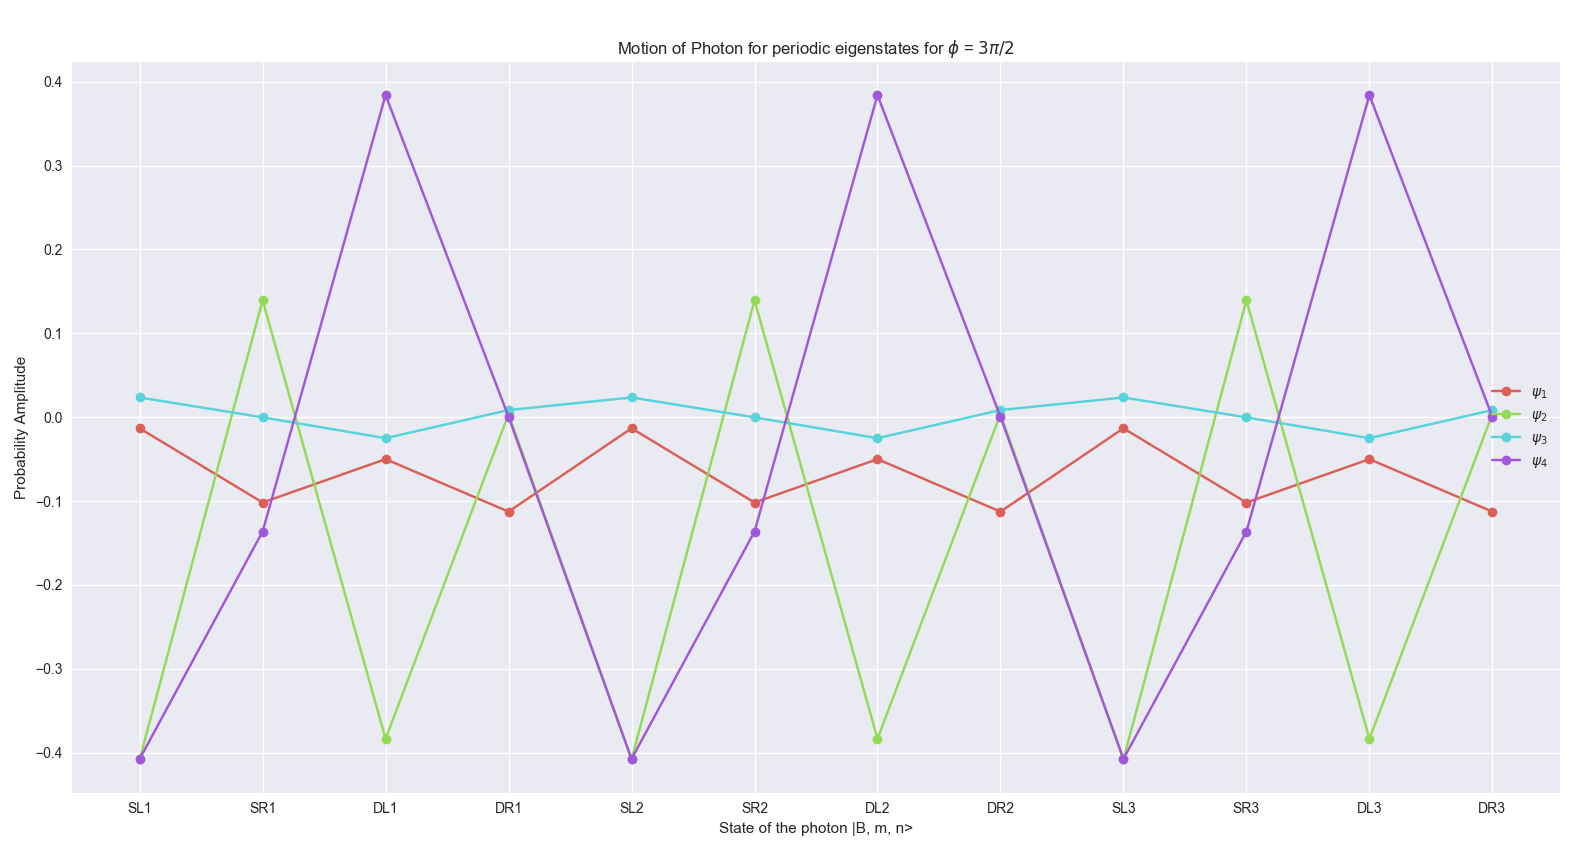
\includegraphics[scale=0.4]{2_Body/Figures/eigenstate_full.png}
    \caption{Probability Amplitudes as a function of the state $\ket{B,M,n}$ of the periodic behaviour Eigenstates for the associated Eigenvalues for the full Hamiltonian evaluated with a multiport phase angle of $3\pi/2$}
    \label{fig:my_label}
\end{figure} 
$\psi_{1}$(red) and $\psi_{2}$(green) belong to the degenerate pair of energy $-\pi/2$ and $\psi_{3}$(blue) and $\psi_{4}$(purple) belong to the degenerate pair of energy $\pi/2$. 

\begin{figure}[H]
    \centering
    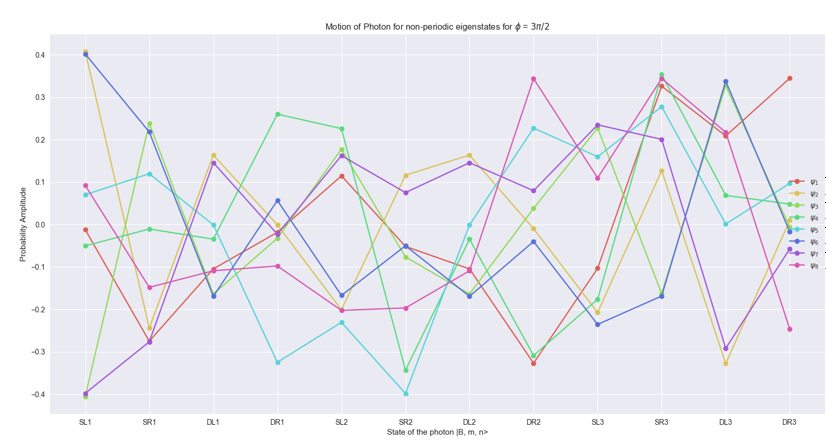
\includegraphics[scale=0.75]{2_Body/Figures/non_periodic_full.png}
    \caption{Probability Amplitudes as a function of the state $\ket{B,M,n}$ of the mixed behaviour Eigenstates for the associated Eigenvalues for a Hamiltonian evaluated with a multiport phase angle of $3\pi/2$}
    \label{fig:my_label}
\end{figure}


\subsection{Qualitative Description}
The four periodic behaving eigenstates exhibit photon transitions between unitcells while maintaining the transition on a fixed bond site and direction of movement. \newline
Given the mixed and random-esque nature of the other eight eigenstates, one cannot deduce any particular pattern of photon movement at those other energy levels. 
\section{Eigenspectrum for Full Hamiltonian}
Numerically we find the full Eigenvalue (Eigenenergy) Spectrum of the Hamiltonian matrix:
\begin{figure}[H]
    \centering
    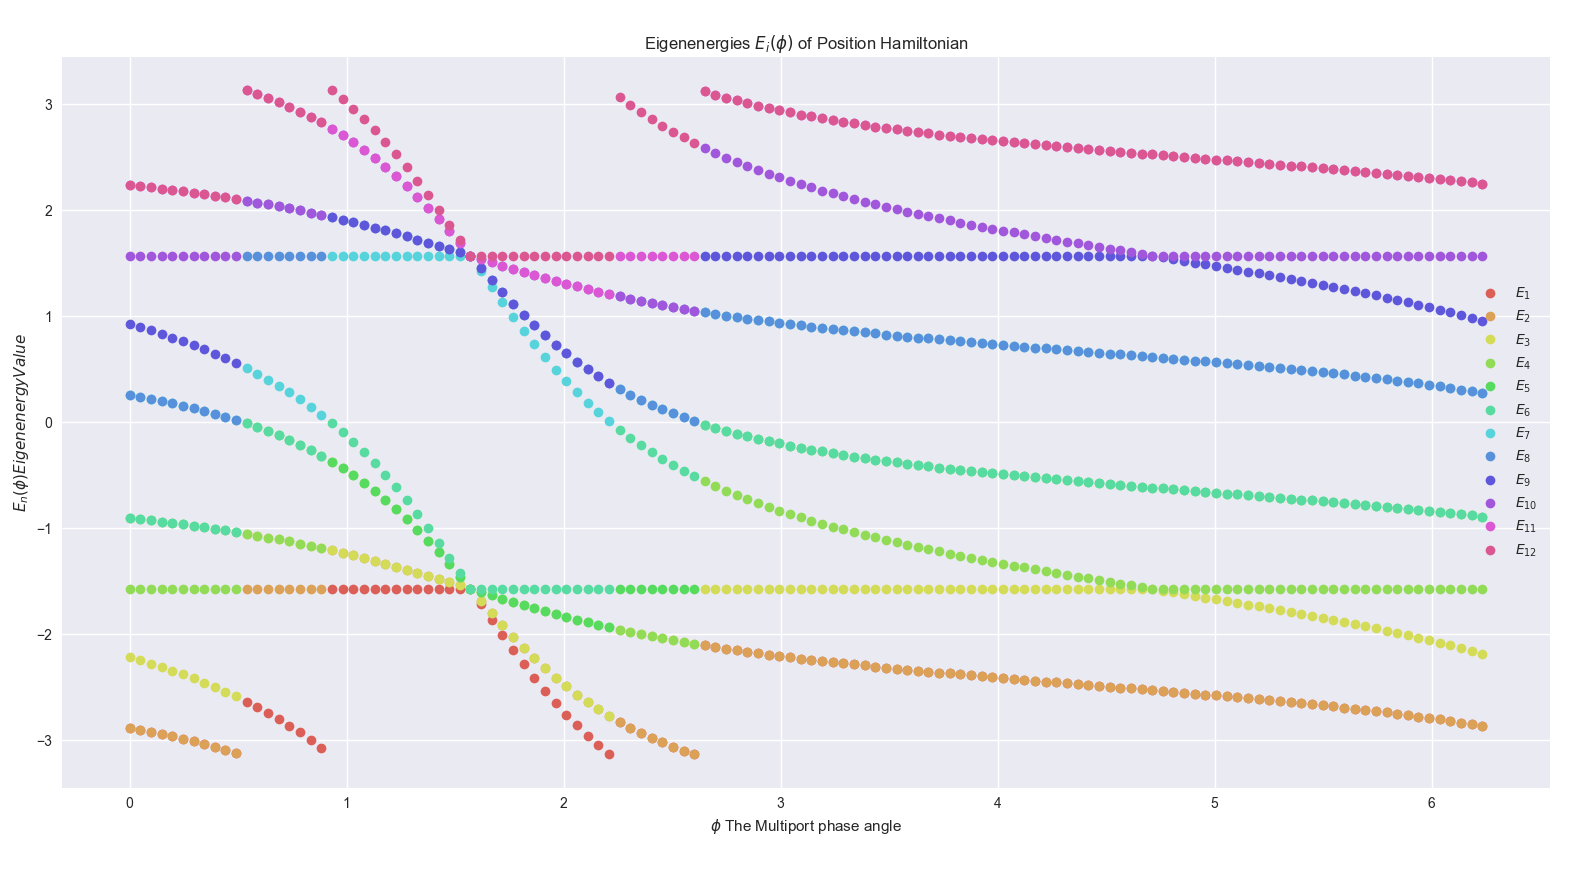
\includegraphics[scale=0.4]{2_Body/Figures/eig_spec_full.png}
    \caption{Eigenvalue/Eigenenergy $E_{i}(\phi)$ spectrum of the full 12 by 12 Hamiltonian (B,M,n) as a function of the multiport phase angle $\phi$}
    \label{fig:my_label}
\end{figure}
\subsection{Discussion}
As revealed earlier, there are two special cases of energy behaviour of the system when the multiport angle is set to $\pi/2$ or $3\pi/2$ which results in a two 6-fold degeneracy system or six 2-fold degeneracy system respectively. 
\newline 
However, for $\phi \neq \frac{k\pi}{2} (k \in \mathbb{Z}$, the system produces a system of four 2-fold degeneracies and eight distinct eigenvalues. \newline
Eigenvalues with a value of $-\pi/2$ always produce an eigenstate that exhibits periodic amplitude behaviour among states (exception being $E=-\pi/2$ for the special case phase angles of $\pi/2, 3\pi/2$). \newline
Other important behaviour include the energy jumps that occur at the following phase angles - $\pi/6, \approx 0.9272,\approx 2.2142,5\pi/6$. \newline
In the case of $\pi/6$ , the twelve eigenvalues converged to $\pi$-multiple values on the unit circle as the multiport phase angle gets closer and closer to $\pi/6$. 
\begin{figure}[H]
    \centering
    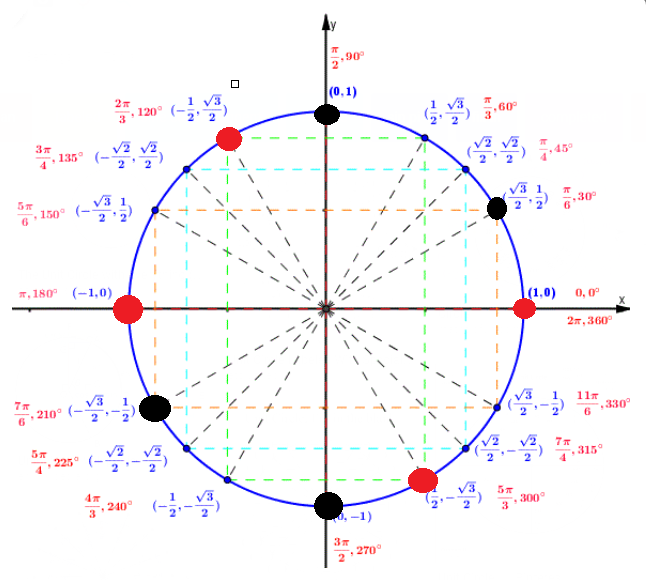
\includegraphics{2_Body/Figures/symmetry_01.png}
    \caption{The eigenvalues the system converges as the multiport phase angle $\phi \rightarrow \pi/6$}
    \label{fig:my_label}
\end{figure}
Red circles denote energies that are 2-fold degenerate and the black circles are non-degenerate energies. It is evident from the convergence of the values before jumping, there's some periodic or cyclic behaviour going on with the energies. If the phase angle becomes $\pi/6$ then the eigenvalues themselves wrap around themselves and are symmetric from each other when it comes positive and negative values. \newline
For example, as $\phi \rightarrow \pi/6$ the values in the following eigenvalues $E_{3} = -5\pi/6, E_{4} = -\pi/2$ shift up when $\phi = \pi/$, we then see the value of $-5\pi/6, -\pi/2$ contained in $E_{1}$ and $E_{2}$. 
\section{Eigenspectrum of Reduced Hamiltonian}
When we use the Hamiltonian that models the energy at the Bond Sites and Unit Cell position given by Eq. 4.36, we get a similar looking Eigenvalue spectrum to that of the full 12 by 12 Hilbert Space Hamiltonian earlier:
\begin{figure}[H]
    \centering
    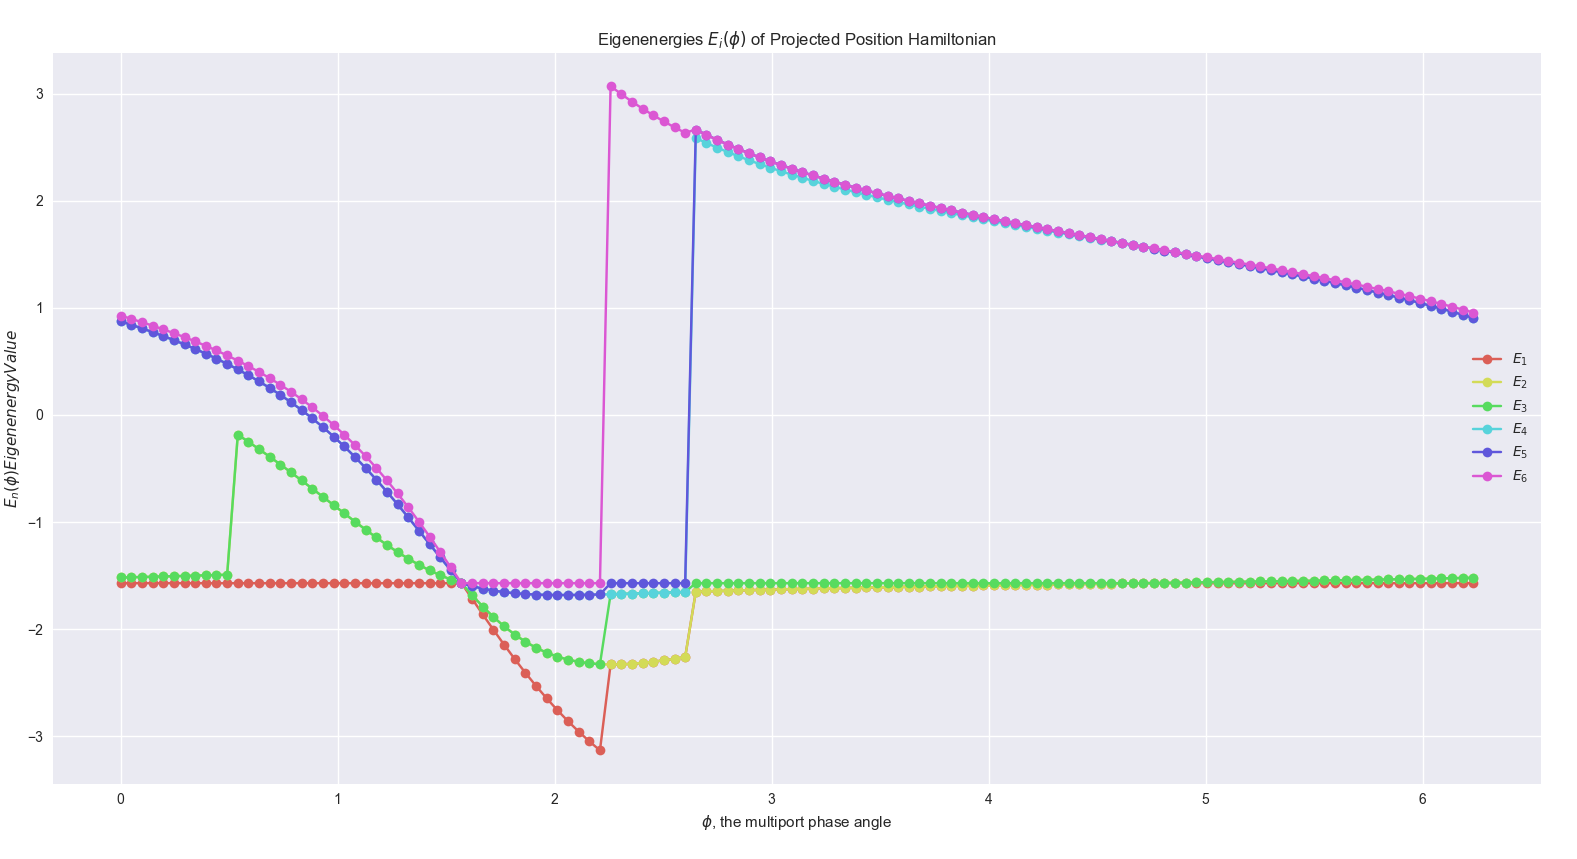
\includegraphics[scale=0.4]{2_Body/reduced_eig_spec.png}
    \caption{Eigenvalue/Eigenenergy spectrum of the projected Hamiltonian (B, n) as a function of the multiport phase angle $\phi$}
    \label{fig:my_label}
\end{figure}
\subsection{Discussion}
The reduced model produces a system with characteristics more similar to that of a Benzene molecule. The Hamiltonian produces a set of two 2-fold degenerate energies and two non-degenerate energies (total of 6 energies) which is analagous to that of the Benzene molecule which produces the same behaviour of degeneracies (see Appendix A.1 for more). \newline
Just like the Full Hamiltonian model, this one produces the same special cases that occur for multiport phase angles of $\pi/2$ and $3\pi/2$. \newline
For $\phi = \pi/2$ , all 6 energies collapse down to a single energy level value of $-\pi/2$ \newline
For $\phi = 3\pi/2$, the 6 energies collapse to a pair of 3-fold degeneracies at values of $-\pi/2$ and $\pi/2$ respectively. \newline
Eigenstates produced by the Reduced Model have a similar pattern to that of the Full Hamiltonian. Once again an energy value of $-\pi/2$ is always an eigenvalue for all $\phi$ and always produces an eigenstate with periodic behaviour for the probability amplitude except for phase angles of $\pi/2, 3\pi/2$ as shown below for a multiport phase angle of $\pi/6$
\begin{figure}[H]
    \centering
    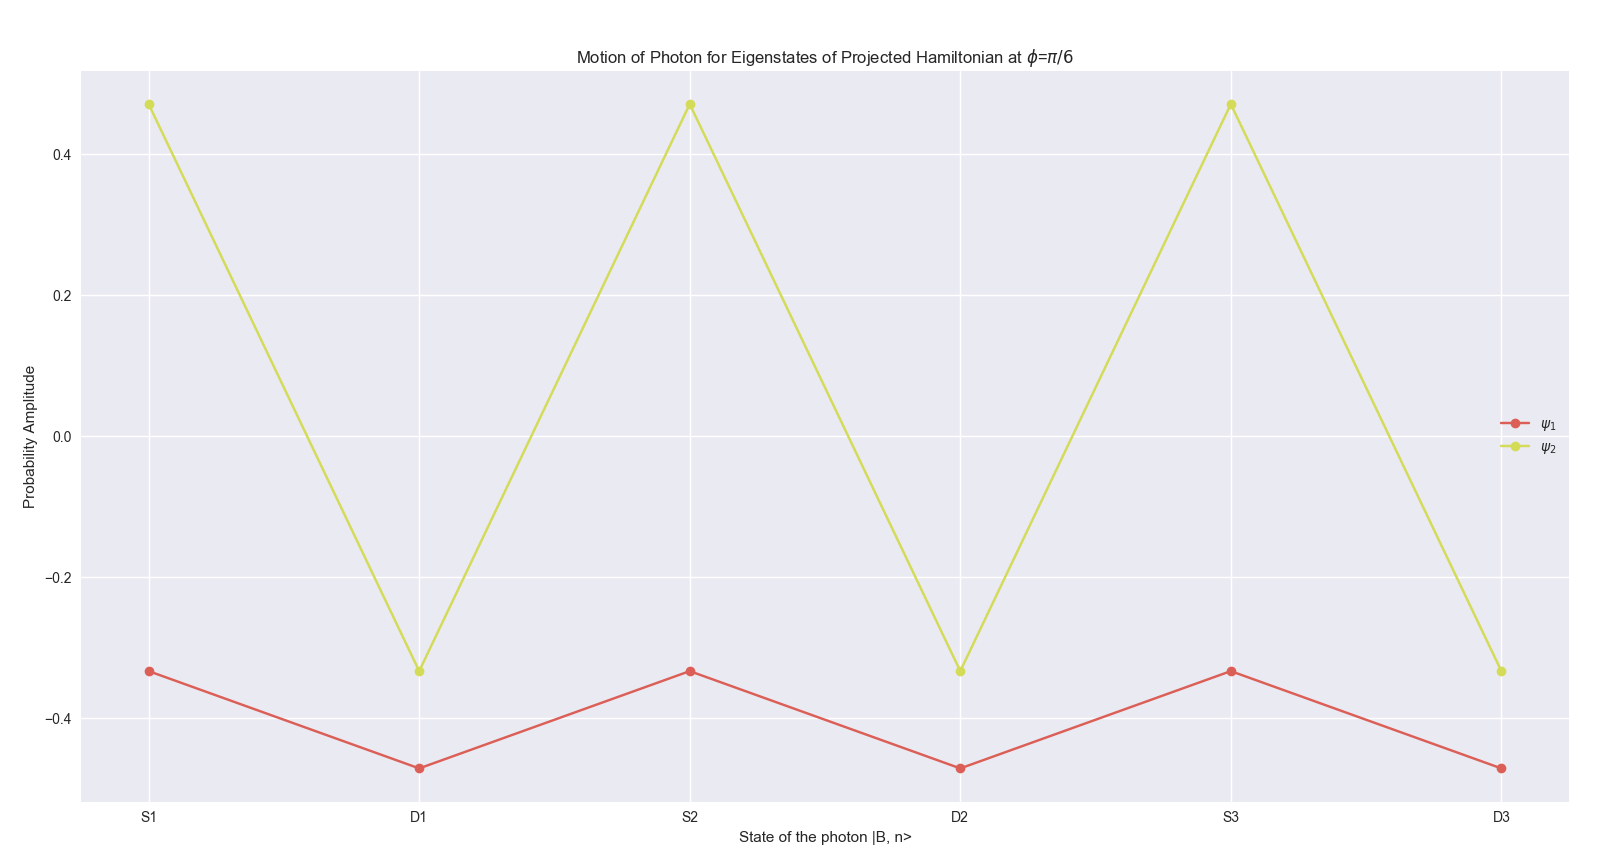
\includegraphics[scale=0.4]{2_Body/red_state.png}
    \caption{Probability Amplitude as a function of the state $\ket{B,M,n}$ of the Periodic Eigenstates for the associated Eigenvalues for a Hamiltonian solved with a multiport phase angle of $\pi/6$ }
    \label{fig:my_label}
\end{figure}

$\psi_{1}$(red) represents $E=-\pi/2$ and $\psi_{2}$ represents $E= \pi/6$. \newline

Periodic eigenstates appear for non-degenerate eigenvalues and all degenerate eigenvalues produce stated with mixed amplitude (no pattern). \newline
The periodic amplitude shows symmetric probability of being within a specific bond site across unit cell jumps (i.e. $S1\rightarrow S2, D2\rightarrow D3$etc.)
Energy jumps in this system occurs at three points of the system at $\pi/6, ~\approx 2.2142, 5\pi/6$ respectively. However, for $\phi = \pi/6$ only energy experiences a jump as opposed to the two occurrences. \newline
Benzene exhibits energies with symmetry of the following approximations (see Appendix A.1 for Huckel Model)
\begin{equation}
    E = \alpha - 2\beta, \alpha - \beta, \alpha + \beta, \alpha + 2\beta
\end{equation}
Where $\alpha, \beta$ are parameters (note: this $\beta$ is different than the one I defined in the model). \newline
The positive-negative symmetry for the Huckel Model of Benzene does not occurs in the interval starting from the last energy jump at $5\pi/6$ which goes on until $E_{3}$ jumps at $\pi/6$. However, the spacing of the energies does not come close to that of the Model and are often within range of folding into 3-fold degeneracy as shown below for the reduced model evaluated at a multiport phase angle of $11\pi/6$
\begin{figure}[H]
    \centering
    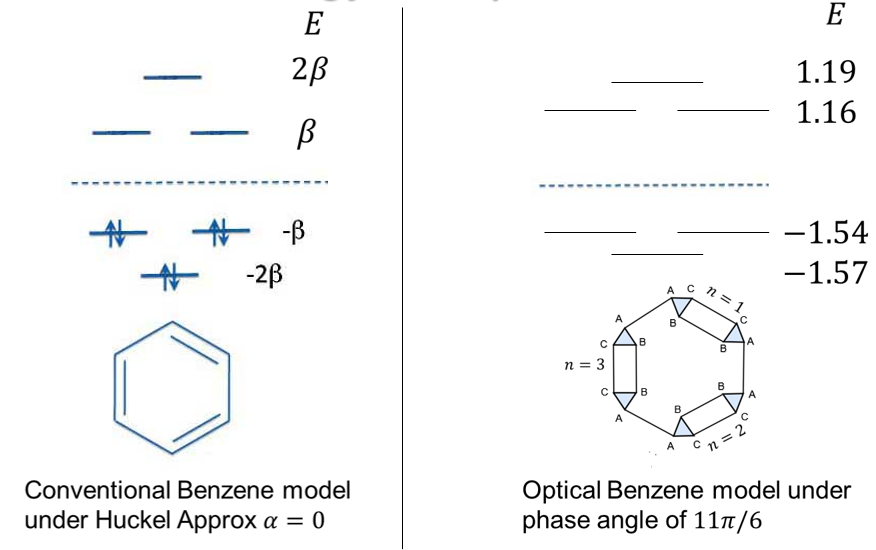
\includegraphics[scale=0.7]{2_Body/energy_comparison.png}
    \caption{Energy Comparison of the Huckel Model of Benzene versus the Optical Benzene model under a phase angle of $11\pi/6$}
    \label{fig:my_label}
\end{figure}